%\documentclass{standalone}
%\usepackage{tikz}
%\usetikzlibrary{patterns,plotmarks}
%\begin{document}
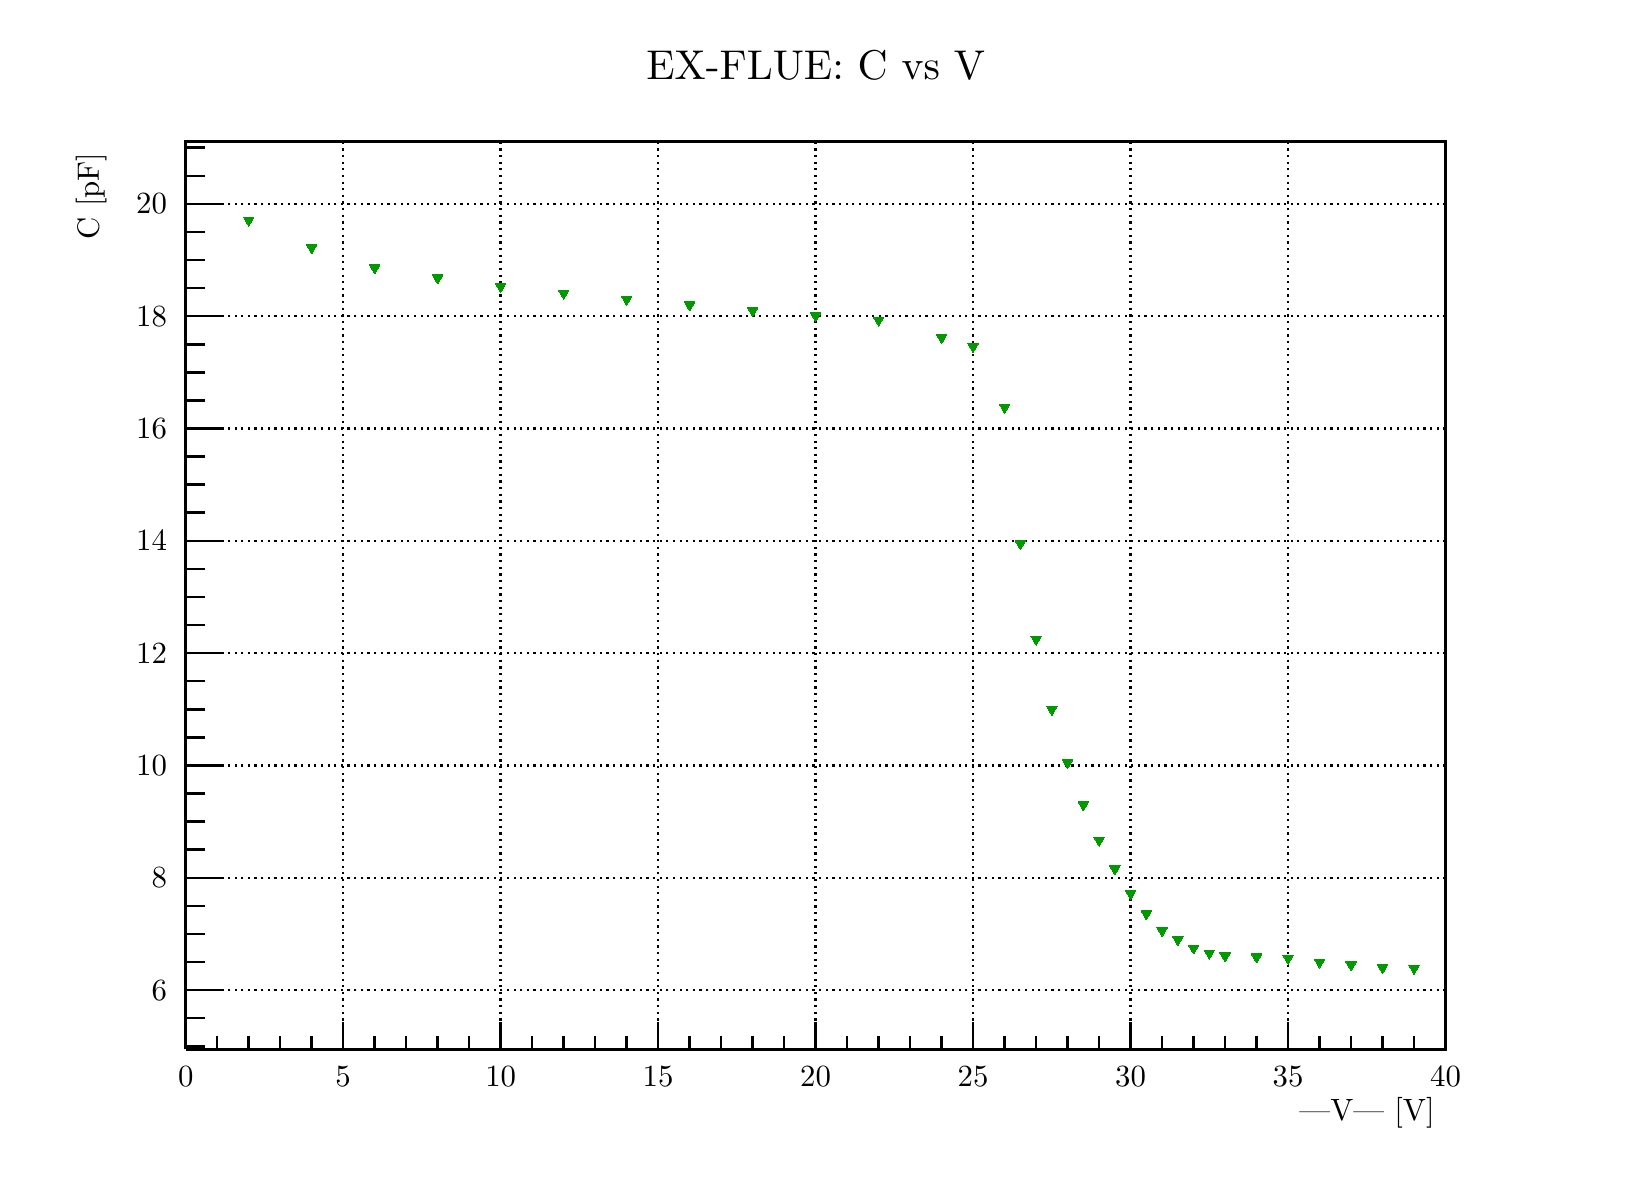
\begin{tikzpicture}
\def\CheckTikzLibraryLoaded#1{ \ifcsname tikz@library@#1@loaded\endcsname \else \PackageWarning{tikz}{usetikzlibrary{#1} is missing in the preamble.} \fi }
\CheckTikzLibraryLoaded{patterns}
\CheckTikzLibraryLoaded{plotmarks}
\pgfdeclareplotmark{cross} {
\pgfpathmoveto{\pgfpoint{-0.3\pgfplotmarksize}{\pgfplotmarksize}}
\pgfpathlineto{\pgfpoint{+0.3\pgfplotmarksize}{\pgfplotmarksize}}
\pgfpathlineto{\pgfpoint{+0.3\pgfplotmarksize}{0.3\pgfplotmarksize}}
\pgfpathlineto{\pgfpoint{+1\pgfplotmarksize}{0.3\pgfplotmarksize}}
\pgfpathlineto{\pgfpoint{+1\pgfplotmarksize}{-0.3\pgfplotmarksize}}
\pgfpathlineto{\pgfpoint{+0.3\pgfplotmarksize}{-0.3\pgfplotmarksize}}
\pgfpathlineto{\pgfpoint{+0.3\pgfplotmarksize}{-1.\pgfplotmarksize}}
\pgfpathlineto{\pgfpoint{-0.3\pgfplotmarksize}{-1.\pgfplotmarksize}}
\pgfpathlineto{\pgfpoint{-0.3\pgfplotmarksize}{-0.3\pgfplotmarksize}}
\pgfpathlineto{\pgfpoint{-1.\pgfplotmarksize}{-0.3\pgfplotmarksize}}
\pgfpathlineto{\pgfpoint{-1.\pgfplotmarksize}{0.3\pgfplotmarksize}}
\pgfpathlineto{\pgfpoint{-0.3\pgfplotmarksize}{0.3\pgfplotmarksize}}
\pgfpathclose
\pgfusepathqstroke
}
\pgfdeclareplotmark{cross*} {
\pgfpathmoveto{\pgfpoint{-0.3\pgfplotmarksize}{\pgfplotmarksize}}
\pgfpathlineto{\pgfpoint{+0.3\pgfplotmarksize}{\pgfplotmarksize}}
\pgfpathlineto{\pgfpoint{+0.3\pgfplotmarksize}{0.3\pgfplotmarksize}}
\pgfpathlineto{\pgfpoint{+1\pgfplotmarksize}{0.3\pgfplotmarksize}}
\pgfpathlineto{\pgfpoint{+1\pgfplotmarksize}{-0.3\pgfplotmarksize}}
\pgfpathlineto{\pgfpoint{+0.3\pgfplotmarksize}{-0.3\pgfplotmarksize}}
\pgfpathlineto{\pgfpoint{+0.3\pgfplotmarksize}{-1.\pgfplotmarksize}}
\pgfpathlineto{\pgfpoint{-0.3\pgfplotmarksize}{-1.\pgfplotmarksize}}
\pgfpathlineto{\pgfpoint{-0.3\pgfplotmarksize}{-0.3\pgfplotmarksize}}
\pgfpathlineto{\pgfpoint{-1.\pgfplotmarksize}{-0.3\pgfplotmarksize}}
\pgfpathlineto{\pgfpoint{-1.\pgfplotmarksize}{0.3\pgfplotmarksize}}
\pgfpathlineto{\pgfpoint{-0.3\pgfplotmarksize}{0.3\pgfplotmarksize}}
\pgfpathclose
\pgfusepathqfillstroke
}
\pgfdeclareplotmark{newstar} {
\pgfpathmoveto{\pgfqpoint{0pt}{\pgfplotmarksize}}
\pgfpathlineto{\pgfqpointpolar{44}{0.5\pgfplotmarksize}}
\pgfpathlineto{\pgfqpointpolar{18}{\pgfplotmarksize}}
\pgfpathlineto{\pgfqpointpolar{-20}{0.5\pgfplotmarksize}}
\pgfpathlineto{\pgfqpointpolar{-54}{\pgfplotmarksize}}
\pgfpathlineto{\pgfqpointpolar{-90}{0.5\pgfplotmarksize}}
\pgfpathlineto{\pgfqpointpolar{234}{\pgfplotmarksize}}
\pgfpathlineto{\pgfqpointpolar{198}{0.5\pgfplotmarksize}}
\pgfpathlineto{\pgfqpointpolar{162}{\pgfplotmarksize}}
\pgfpathlineto{\pgfqpointpolar{134}{0.5\pgfplotmarksize}}
\pgfpathclose
\pgfusepathqstroke
}
\pgfdeclareplotmark{newstar*} {
\pgfpathmoveto{\pgfqpoint{0pt}{\pgfplotmarksize}}
\pgfpathlineto{\pgfqpointpolar{44}{0.5\pgfplotmarksize}}
\pgfpathlineto{\pgfqpointpolar{18}{\pgfplotmarksize}}
\pgfpathlineto{\pgfqpointpolar{-20}{0.5\pgfplotmarksize}}
\pgfpathlineto{\pgfqpointpolar{-54}{\pgfplotmarksize}}
\pgfpathlineto{\pgfqpointpolar{-90}{0.5\pgfplotmarksize}}
\pgfpathlineto{\pgfqpointpolar{234}{\pgfplotmarksize}}
\pgfpathlineto{\pgfqpointpolar{198}{0.5\pgfplotmarksize}}
\pgfpathlineto{\pgfqpointpolar{162}{\pgfplotmarksize}}
\pgfpathlineto{\pgfqpointpolar{134}{0.5\pgfplotmarksize}}
\pgfpathclose
\pgfusepathqfillstroke
}
\definecolor{c}{rgb}{1,1,1};
\draw [color=c, fill=c] (0,0) rectangle (20,14.411);
\draw [color=c, fill=c] (2,1.4411) rectangle (18,12.9699);
\definecolor{c}{rgb}{0,0,0};
\draw [c,line width=0.9] (2,1.4411) -- (2,12.9699) -- (18,12.9699) -- (18,1.4411) -- (2,1.4411);
\definecolor{c}{rgb}{1,1,1};
\draw [color=c, fill=c] (2,1.4411) rectangle (18,12.9699);
\definecolor{c}{rgb}{0,0,0};
\draw [c,line width=0.9] (2,1.4411) -- (2,12.9699) -- (18,12.9699) -- (18,1.4411) -- (2,1.4411);
\draw [c,line width=0.9] (2,1.4411) -- (18,1.4411);
\draw [c,dash pattern=on 0.80pt off 1.60pt ,line width=0.9] (2,12.9699) -- (2,1.4411);
\draw [c,dash pattern=on 0.80pt off 1.60pt ,line width=0.9] (4,12.9699) -- (4,1.4411);
\draw [c,dash pattern=on 0.80pt off 1.60pt ,line width=0.9] (6,12.9699) -- (6,1.4411);
\draw [c,dash pattern=on 0.80pt off 1.60pt ,line width=0.9] (8,12.9699) -- (8,1.4411);
\draw [c,dash pattern=on 0.80pt off 1.60pt ,line width=0.9] (10,12.9699) -- (10,1.4411);
\draw [c,dash pattern=on 0.80pt off 1.60pt ,line width=0.9] (12,12.9699) -- (12,1.4411);
\draw [c,dash pattern=on 0.80pt off 1.60pt ,line width=0.9] (14,12.9699) -- (14,1.4411);
\draw [c,dash pattern=on 0.80pt off 1.60pt ,line width=0.9] (16,12.9699) -- (16,1.4411);
\draw [c,dash pattern=on 0.80pt off 1.60pt ,line width=0.9] (18,12.9699) -- (18,1.4411);
\draw [c,line width=0.9] (2,1.4411) -- (2,12.9699);
\draw [c,dash pattern=on 0.80pt off 1.60pt ,line width=0.9] (18,2.195) -- (2,2.195);
\draw [c,dash pattern=on 0.80pt off 1.60pt ,line width=0.9] (18,3.62148) -- (2,3.62148);
\draw [c,dash pattern=on 0.80pt off 1.60pt ,line width=0.9] (18,5.04796) -- (2,5.04796);
\draw [c,dash pattern=on 0.80pt off 1.60pt ,line width=0.9] (18,6.47444) -- (2,6.47444);
\draw [c,dash pattern=on 0.80pt off 1.60pt ,line width=0.9] (18,7.90092) -- (2,7.90092);
\draw [c,dash pattern=on 0.80pt off 1.60pt ,line width=0.9] (18,9.3274) -- (2,9.3274);
\draw [c,dash pattern=on 0.80pt off 1.60pt ,line width=0.9] (18,10.7539) -- (2,10.7539);
\draw [c,dash pattern=on 0.80pt off 1.60pt ,line width=0.9] (18,12.1804) -- (2,12.1804);
\draw [c,dash pattern=on 0.80pt off 1.60pt ,line width=0.9] (18,2.195) -- (2,2.195);
\draw [c,dash pattern=on 0.80pt off 1.60pt ,line width=0.9] (18,12.1804) -- (2,12.1804);
\draw [c,line width=0.9] (2,1.4411) -- (18,1.4411);
\draw [c,line width=0.9] (2,1.78697) -- (2,1.4411);
\draw [c,line width=0.9] (2.4,1.61404) -- (2.4,1.4411);
\draw [c,line width=0.9] (2.8,1.61404) -- (2.8,1.4411);
\draw [c,line width=0.9] (3.2,1.61404) -- (3.2,1.4411);
\draw [c,line width=0.9] (3.6,1.61404) -- (3.6,1.4411);
\draw [c,line width=0.9] (4,1.78697) -- (4,1.4411);
\draw [c,line width=0.9] (4.4,1.61404) -- (4.4,1.4411);
\draw [c,line width=0.9] (4.8,1.61404) -- (4.8,1.4411);
\draw [c,line width=0.9] (5.2,1.61404) -- (5.2,1.4411);
\draw [c,line width=0.9] (5.6,1.61404) -- (5.6,1.4411);
\draw [c,line width=0.9] (6,1.78697) -- (6,1.4411);
\draw [c,line width=0.9] (6.4,1.61404) -- (6.4,1.4411);
\draw [c,line width=0.9] (6.8,1.61404) -- (6.8,1.4411);
\draw [c,line width=0.9] (7.2,1.61404) -- (7.2,1.4411);
\draw [c,line width=0.9] (7.6,1.61404) -- (7.6,1.4411);
\draw [c,line width=0.9] (8,1.78697) -- (8,1.4411);
\draw [c,line width=0.9] (8.4,1.61404) -- (8.4,1.4411);
\draw [c,line width=0.9] (8.8,1.61404) -- (8.8,1.4411);
\draw [c,line width=0.9] (9.2,1.61404) -- (9.2,1.4411);
\draw [c,line width=0.9] (9.6,1.61404) -- (9.6,1.4411);
\draw [c,line width=0.9] (10,1.78697) -- (10,1.4411);
\draw [c,line width=0.9] (10.4,1.61404) -- (10.4,1.4411);
\draw [c,line width=0.9] (10.8,1.61404) -- (10.8,1.4411);
\draw [c,line width=0.9] (11.2,1.61404) -- (11.2,1.4411);
\draw [c,line width=0.9] (11.6,1.61404) -- (11.6,1.4411);
\draw [c,line width=0.9] (12,1.78697) -- (12,1.4411);
\draw [c,line width=0.9] (12.4,1.61404) -- (12.4,1.4411);
\draw [c,line width=0.9] (12.8,1.61404) -- (12.8,1.4411);
\draw [c,line width=0.9] (13.2,1.61404) -- (13.2,1.4411);
\draw [c,line width=0.9] (13.6,1.61404) -- (13.6,1.4411);
\draw [c,line width=0.9] (14,1.78697) -- (14,1.4411);
\draw [c,line width=0.9] (14.4,1.61404) -- (14.4,1.4411);
\draw [c,line width=0.9] (14.8,1.61404) -- (14.8,1.4411);
\draw [c,line width=0.9] (15.2,1.61404) -- (15.2,1.4411);
\draw [c,line width=0.9] (15.6,1.61404) -- (15.6,1.4411);
\draw [c,line width=0.9] (16,1.78697) -- (16,1.4411);
\draw [c,line width=0.9] (16.4,1.61404) -- (16.4,1.4411);
\draw [c,line width=0.9] (16.8,1.61404) -- (16.8,1.4411);
\draw [c,line width=0.9] (17.2,1.61404) -- (17.2,1.4411);
\draw [c,line width=0.9] (17.6,1.61404) -- (17.6,1.4411);
\draw [c,line width=0.9] (18,1.78697) -- (18,1.4411);
\draw [anchor=base] (2,0.965539) node[scale=1.11327, color=c, rotate=0]{0};
\draw [anchor=base] (4,0.965539) node[scale=1.11327, color=c, rotate=0]{5};
\draw [anchor=base] (6,0.965539) node[scale=1.11327, color=c, rotate=0]{10};
\draw [anchor=base] (8,0.965539) node[scale=1.11327, color=c, rotate=0]{15};
\draw [anchor=base] (10,0.965539) node[scale=1.11327, color=c, rotate=0]{20};
\draw [anchor=base] (12,0.965539) node[scale=1.11327, color=c, rotate=0]{25};
\draw [anchor=base] (14,0.965539) node[scale=1.11327, color=c, rotate=0]{30};
\draw [anchor=base] (16,0.965539) node[scale=1.11327, color=c, rotate=0]{35};
\draw [anchor=base] (18,0.965539) node[scale=1.11327, color=c, rotate=0]{40};
\draw [anchor= east] (18,0.634085) node[scale=1.11327, color=c, rotate=0]{|V| [V]};
\draw [c,line width=0.9] (2,1.4411) -- (2,12.9699);
\draw [c,line width=0.9] (2.48,2.195) -- (2,2.195);
\draw [c,line width=0.9] (2.24,2.55162) -- (2,2.55162);
\draw [c,line width=0.9] (2.24,2.90824) -- (2,2.90824);
\draw [c,line width=0.9] (2.24,3.26486) -- (2,3.26486);
\draw [c,line width=0.9] (2.48,3.62148) -- (2,3.62148);
\draw [c,line width=0.9] (2.24,3.9781) -- (2,3.9781);
\draw [c,line width=0.9] (2.24,4.33472) -- (2,4.33472);
\draw [c,line width=0.9] (2.24,4.69134) -- (2,4.69134);
\draw [c,line width=0.9] (2.48,5.04796) -- (2,5.04796);
\draw [c,line width=0.9] (2.24,5.40458) -- (2,5.40458);
\draw [c,line width=0.9] (2.24,5.7612) -- (2,5.7612);
\draw [c,line width=0.9] (2.24,6.11782) -- (2,6.11782);
\draw [c,line width=0.9] (2.48,6.47444) -- (2,6.47444);
\draw [c,line width=0.9] (2.24,6.83106) -- (2,6.83106);
\draw [c,line width=0.9] (2.24,7.18768) -- (2,7.18768);
\draw [c,line width=0.9] (2.24,7.5443) -- (2,7.5443);
\draw [c,line width=0.9] (2.48,7.90092) -- (2,7.90092);
\draw [c,line width=0.9] (2.24,8.25754) -- (2,8.25754);
\draw [c,line width=0.9] (2.24,8.61416) -- (2,8.61416);
\draw [c,line width=0.9] (2.24,8.97078) -- (2,8.97078);
\draw [c,line width=0.9] (2.48,9.3274) -- (2,9.3274);
\draw [c,line width=0.9] (2.24,9.68402) -- (2,9.68402);
\draw [c,line width=0.9] (2.24,10.0406) -- (2,10.0406);
\draw [c,line width=0.9] (2.24,10.3973) -- (2,10.3973);
\draw [c,line width=0.9] (2.48,10.7539) -- (2,10.7539);
\draw [c,line width=0.9] (2.24,11.1105) -- (2,11.1105);
\draw [c,line width=0.9] (2.24,11.4671) -- (2,11.4671);
\draw [c,line width=0.9] (2.24,11.8237) -- (2,11.8237);
\draw [c,line width=0.9] (2.48,12.1804) -- (2,12.1804);
\draw [c,line width=0.9] (2.48,2.195) -- (2,2.195);
\draw [c,line width=0.9] (2.24,1.83838) -- (2,1.83838);
\draw [c,line width=0.9] (2.24,1.48176) -- (2,1.48176);
\draw [c,line width=0.9] (2.48,12.1804) -- (2,12.1804);
\draw [c,line width=0.9] (2.24,12.537) -- (2,12.537);
\draw [c,line width=0.9] (2.24,12.8936) -- (2,12.8936);
\draw [anchor= east] (1.9,2.195) node[scale=1.11327, color=c, rotate=0]{6};
\draw [anchor= east] (1.9,3.62148) node[scale=1.11327, color=c, rotate=0]{8};
\draw [anchor= east] (1.9,5.04796) node[scale=1.11327, color=c, rotate=0]{10};
\draw [anchor= east] (1.9,6.47444) node[scale=1.11327, color=c, rotate=0]{12};
\draw [anchor= east] (1.9,7.90092) node[scale=1.11327, color=c, rotate=0]{14};
\draw [anchor= east] (1.9,9.3274) node[scale=1.11327, color=c, rotate=0]{16};
\draw [anchor= east] (1.9,10.7539) node[scale=1.11327, color=c, rotate=0]{18};
\draw [anchor= east] (1.9,12.1804) node[scale=1.11327, color=c, rotate=0]{20};
\draw [anchor= east] (0.798747,12.9699) node[scale=1.11327, color=c, rotate=90]{C [pF]};
\definecolor{c}{rgb}{0,0.6,0};
\foreach \P in {(2.8,11.9735), (3.6,11.624), (4.4,11.3673), (5.2,11.2389), (6,11.1319), (6.8,11.0463), (7.6,10.9679), (8.4,10.8965), (9.2,10.8252), (10,10.761), (10.8,10.704), (11.6,10.4829), (12,10.3687), (12.4,9.59844), (12.6,7.86526),
 (12.8,6.65275), (13,5.7612), (13.2,5.08362), (13.4,4.54869), (13.6,4.09935), (13.8,3.7356), (14,3.42177), (14.2,3.16501), (14.4,2.95103), (14.6,2.83691), (14.8,2.72993), (15,2.66574), (15.2,2.63007), (15.6,2.61581), (16,2.60155), (16.4,2.55162),
 (16.8,2.51596), (17.2,2.48029), (17.6,2.47316)}{\draw[mark options={color=c,fill=c,rotate=180},mark size=2.162162pt, line width=0.000000pt, mark=triangle*] plot coordinates {\P};}
\definecolor{c}{rgb}{0,0,0};
\draw (10,13.9427) node[scale=1.50291, color=c, rotate=0]{EX-FLUE: C vs V};
\end{tikzpicture}
%\end{document}
